% This is samplepaper.tex, a sample chapter demonstrating the
% LLNCS macro package for Springer Computer Science proceedings;
% Version 2.20 of 2017/10/04
%

\documentclass[runningheads]{llncs}
\usepackage{multirow}
\usepackage{graphicx}
\usepackage{float}
\usepackage{caption}
\usepackage{subcaption}


% Used for displaying a sample figure. If possible, figure files should
% be included in EPS format.
%
% If you use the hyperref package, please uncomment the following line
% to display URLs in blue roman font according to Springer's eBook style:
% \renewcommand\UrlFont{\color{blue}\rmfamily}

\begin{document}
%
\title{Investigation of the Impact of Mobility on Multi-Hop Packet Transmission in a Bicycle Network}
%
%\titlerunning{Abbreviated paper title}
% If the paper title is too long for the running head, you can set
% an abbreviated paper title here
%
\author{António Nunes Duarte \and
Sarah Wu \and
Umer Iqbal} % TODO: His name
%
% \authorrunning{F. Author et al.}
% First names are abbreviated in the running head.
% If there are more than two authors, 'et al.' is used.
%
\institute{TU Dresden}
%

\titlerunning{Multi-Hop Packet Transmission in a Bicycle Network}
\maketitle              % typeset the header of the contribution
%
%\begin{abstract}
%Causal replication is a weak consistency model, that works by 
%tracking causal dependencies between operations of a system and making sure that they are propagated
%and displayed, to users of that system, in a causally consistent order.
%Many ways of achieving causal consistency have been proposed in the literature
%over the years, (e.g.
%usage of Logical Clocks\cite{baquero2016logical},
%Logical Clocks with Physical Timestamps\cite{roohitavaf2017causalspartan,du2014gentlerain}, tracking Direct Dependencies\cite{lloyd2011don}, 
%	usage of specific node topologies that naturally ensure consistency\cite{van2020intrinsic})
%but each comes with it's own set of trade-offs which turn the decision complicated 
%and	highly dependent on the specification of the system that one is looking to develop.
%The aim of this work, is
%exploring those trade-offs through the usage of a simulator, to more thoroughly understand the limits,
%and optimal use cases of each proposed solution.

%\keywords{Causality Tracking \and Consistency \and Simulator}
%\end{abstract}

\section{Introduction}

Wireless Sensor Networks (WSNs) have received significant attention in recent years due to their wide range of applications, including environmental monitoring, healthcare, smart cities, and military surveillance. A key characteristic of WSNs is their ability to operate unattended in various environments, capturing and transmitting data over potentially long distances.

A challenging scenario for WSNs involves deploying sensors on mobile platforms, such as bicycles or cars, where node mobility can significantly affect the network's performance. This report presents an investigation into the impact of mobility on multi-hop packet transmission within a WSN, with a focus on a bicycle network scenario. In particular, we examine the effect of various parameters, including inter-packet interval (IPI), packet size, distance between bicycles, speed of bicycles, transmission channel, and transmission power on the packet success rate.

Our experimental setup includes three bicycles equipped with wireless sensor nodes, moving in a linear arrangement. The extreme nodes communicate via burst transmission, with the middle node serving as a relay. The primary aim of this investigation is to gain insights into the effects of these parameters on the packet transmission quality, as quantified by the Link Quality Indicator (LQI) and Received Signal Strength Indicator (RSSI) values. The findings are anticipated to provide valuable guidance for the design and operation of mobile WSNs.

\clearpage

% \section{Related Work}

\section{Implementation}

The Contiki-NG operating system, an open-source, highly portable multitasking operating system for memory-efficient networked embedded systems and wireless sensor networks, was used to set up and analyze the wireless sensor networks. This choice was motivated by Contiki-NG's low memory footprint, its modular architecture that allows for easy configuration, and its strong support for network simulations.

We implemented three distinct processes within the Contiki-NG environment:

\begin{itemize}
    \item \textbf{End Process}: This process runs on the sender nodes at the ends of the bicycle chain. It is implemented as a periodic timer, which sends a packet every IPI. The packets consist of a message ID and a payload, which are generated by the \texttt{generate\_message} function. The message ID is used for tracking the packets, while the payload consists of repeated characters for simplicity. When a packet is received, it is logged into a file in the node's flash memory, along with the Link Quality Indicator (LQI) and the Received Signal Strength Indicator (RSSI). The LQI and RSSI provide measures of the packet transmission quality.
    \item \textbf{Relay Process}: This process runs on the relay node. Upon receiving a packet from an end node, it immediately forwards the packet to the other end node. The relay process uses the \texttt{udp\_rx\_callback} function to receive and forward packets. To ensure that the packets are forwarded correctly, the relay process keeps track of the IP addresses of the end nodes. This process is critical to enabling multi-hop packet transmission in the bicycle network.
    \item \textbf{Transfer Process}: This is an auxiliary process that is used for transferring the log files from the end nodes to a connected computer via the USB serial interface. This process is activated by pressing the user button on the end node. The log files contain the LQI and RSSI values for each packet received, which are later used for analyzing the packet transmission quality.
    \end{itemize}

    \clearpage
    

\section{Experimental Setup}

For our experimental setup, as defined in the objectives of the project, we used three Zolertia Remote Revision B wireless sensor nodes. The nodes were placed on three bicycles, with the middle node acting as a relay between the two end nodes. The nodes were placed in a linear arrangement, with the distance between the end nodes being initially approximately 10 meters.
The nodes were powered each through it's own Raspberry Pi, which was itself connected to a battery bank.
After experimenting with each parameter, we would extract the log results from each node. Then, we would analyze them to determine the impact of the new parameter on the results before reflashing the nodes with a new configuration.

The chosen configuration values can be observed in Table~\ref{table:1}.

\vspace{0.5cm}

\begin{table}[h!]
    \centering
    \begin{tabular}{| c|c| c| c|} 
    \hline
     \textbf{Test} & \textbf{Packet Size} & \textbf{TX Power} & \textbf{TX Channel} \\ [0.5ex] 
    \hline
     1 & 50 (default) & 0 (default) & 26 (default) \\ 
     \hline
     2 & 50 (default) & -12 & 26 (default) \\
     \hline
     3 & 50 (default) & -24 & 26 (default) \\
     \hline
     4 & 50 (default) & 7 & 26 (default) \\
     \hline
     5 & 50 (default) & 0 (default) & 11 \\
     \hline
     6 & 50 (default) & 0 (default) & 15 \\
     \hline
     7 & 50 (default) & 0 (default) & 20 \\
     \hline
     8 & 20  & 0 (default) & 26 (default) \\
     \hline
     9 & 100 & 0 (default) & 26 (default) \\
     \hline
    \end{tabular}
    \vspace*{0.2cm}
    \caption{Test configuration parameters.}
    \label{table:1}
    \end{table}

We also tested increasing or decreasing the speed of the bikes, as well as the distance between them, but due to inaccuracies in the measurement of those parameters (and probably changes in the surrounding environments while we conducted the tests), we were unable to draw any reasonable conclusions from those variations. We did, however, notice that both speed and distance did seem to generally cause the values of LQI and RSSI to decrease, although we couldn't be accurate enough in order for the results to be easily reproducible and reliable.

A rough diagram of the setup can be observed in Figure~\ref{fig:1}.

\vspace{0.5cm}

\begin{figure}[H]
    \centering
    \begin{subfigure}[b]{0.45\textwidth}
        \centering
        
\includegraphics[width=\textwidth]{images/bike-diagram-cropped.pdf}
    \end{subfigure}
    \caption{Bike Arrangement}
    \label{fig:1}
\end{figure}

\clearpage

\section{Results}

In order to display the results in a more readable manner, we analyzed the data and produced several plots for each configuration.

We display the results of each configuration as both a line plot, and a histogram plot. The line plot displays the LQI and RSSI values for each packet received, while the histogram plot displays the distribution of the LQI and RSSI values for all packets received.

\vspace{0.3cm}

\begin{figure}[ht]
    \centering
    \begin{subfigure}[b]{0.45\textwidth}
        \centering
        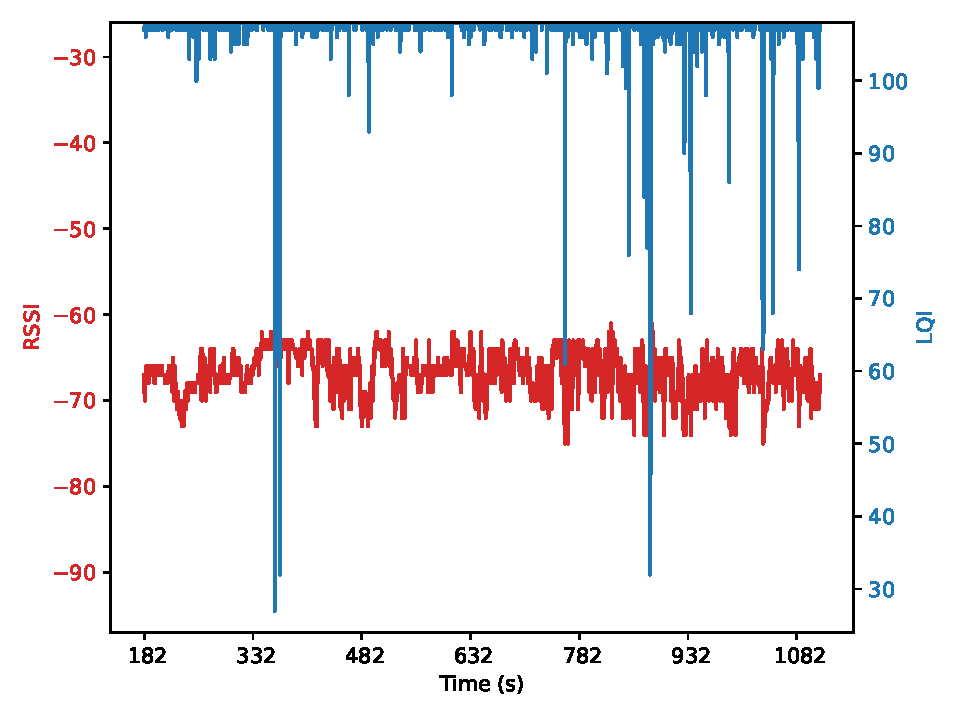
\includegraphics[width=\textwidth]{images/1-50-0-26-line.pdf}
        \caption{Line plot}
    \end{subfigure}
    \hfill
    \begin{subfigure}[b]{0.45\textwidth}
        \centering
        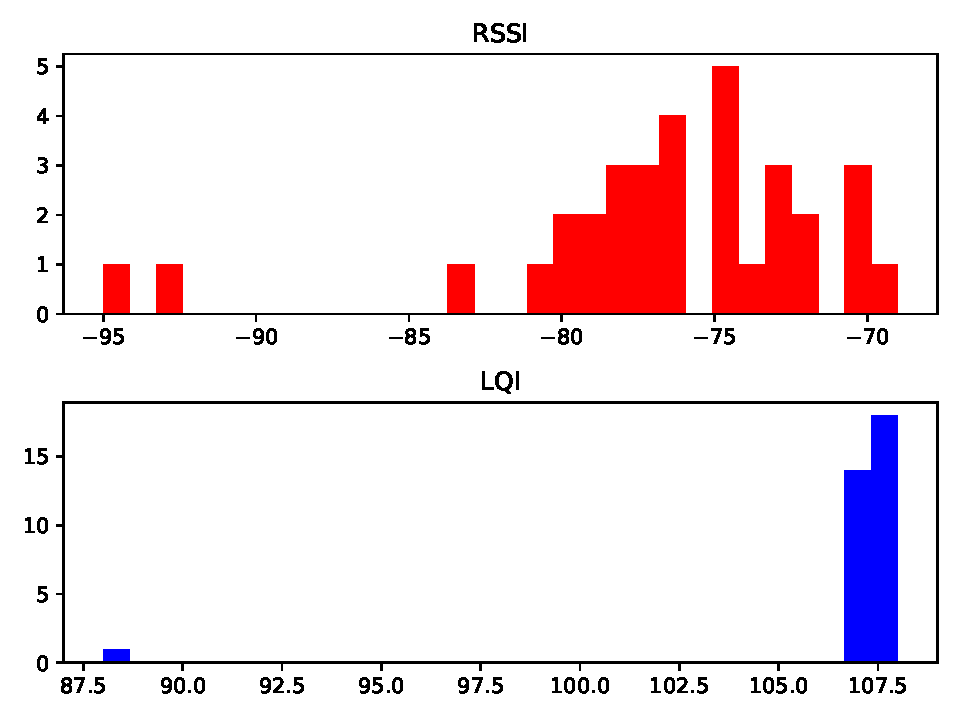
\includegraphics[width=\textwidth]{images/1-50-0-26-histogram.pdf}
        \caption{Histogram plot}
    \end{subfigure}
    \caption{Plots for Test 1}
\end{figure}

\begin{figure}[ht]
    \centering
    \begin{subfigure}[b]{0.45\textwidth}
        \centering
        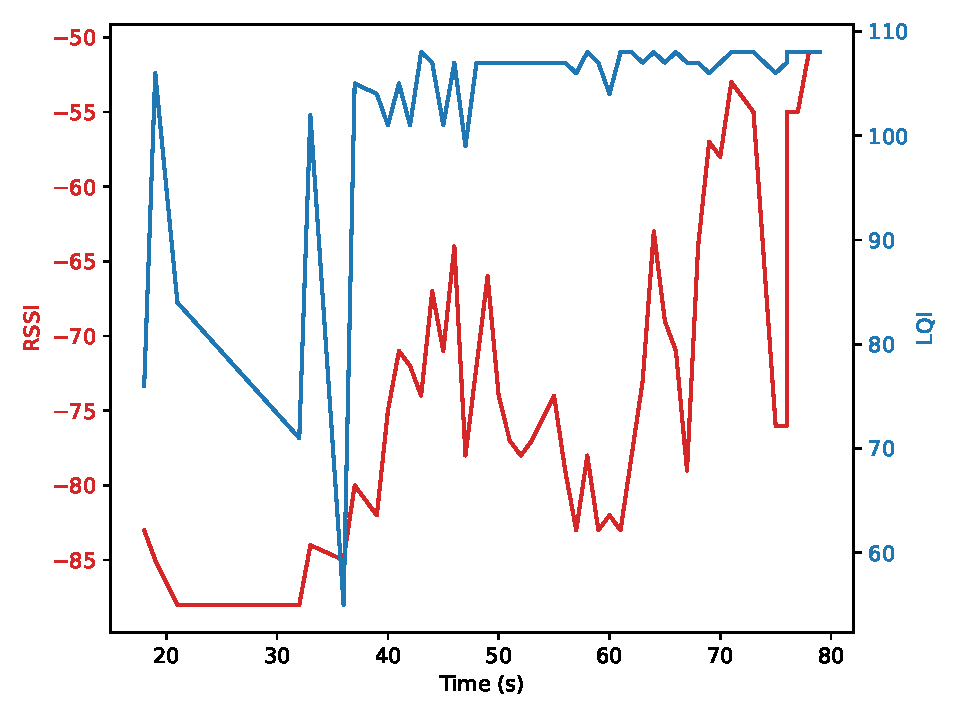
\includegraphics[width=\textwidth]{images/1-50--12-26-line.pdf}
        \caption{Line plot}
    \end{subfigure}
    \hfill
    \begin{subfigure}[b]{0.45\textwidth}
        \centering
        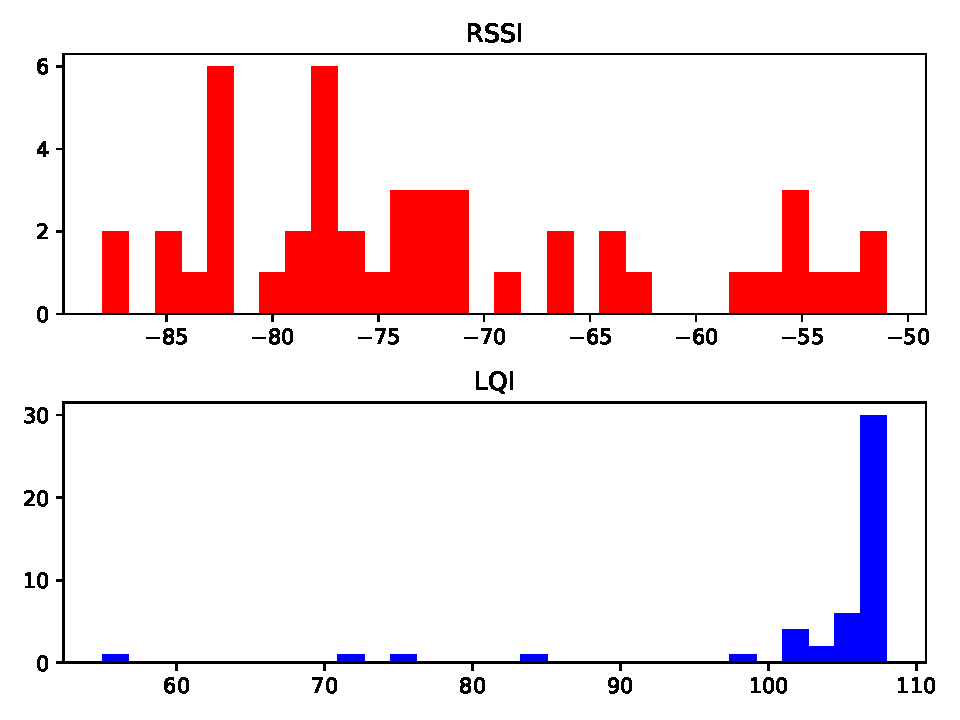
\includegraphics[width=\textwidth]{images/1-50--12-26-histogram.pdf}
        \caption{Histogram plot}
    \end{subfigure}
    \caption{Plots for Test 2}
\end{figure}

\begin{figure}[ht]
    \centering
    \begin{subfigure}[b]{0.45\textwidth}
        \centering
        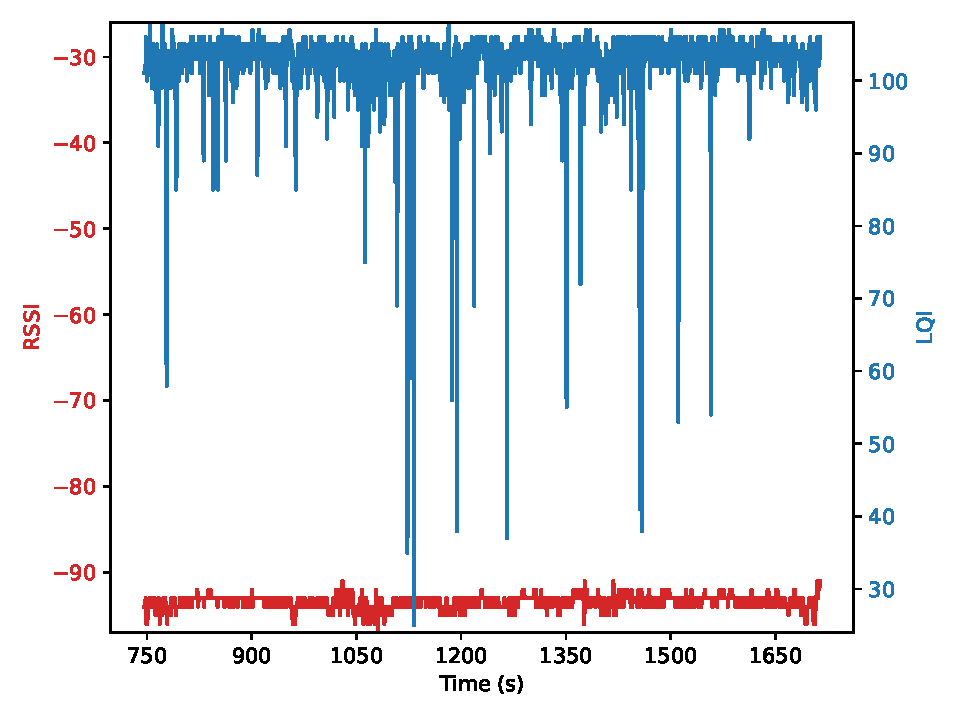
\includegraphics[width=\textwidth]{images/1-50--24-26-line.pdf}
        \caption{Line plot}
    \end{subfigure}
    \hfill
    \begin{subfigure}[b]{0.45\textwidth}
        \centering
        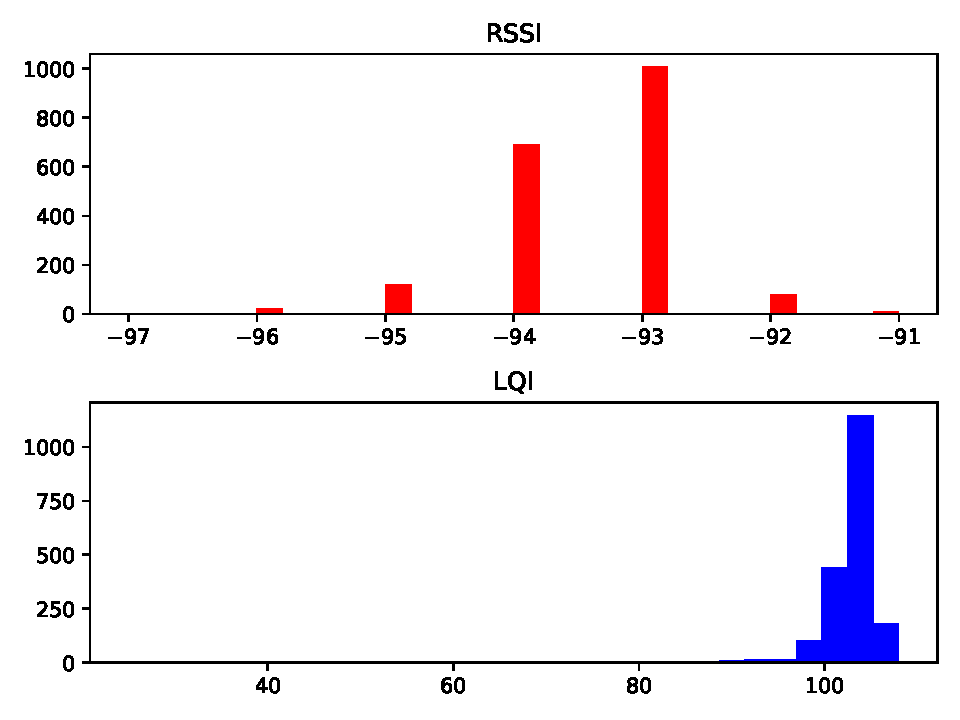
\includegraphics[width=\textwidth]{images/1-50--24-26-histogram.pdf}
        \caption{Histogram plot}
    \end{subfigure}
    \caption{Plots for Test 3}
\end{figure}

\begin{figure}[ht]
    \centering
    \begin{subfigure}[b]{0.45\textwidth}
        \centering
        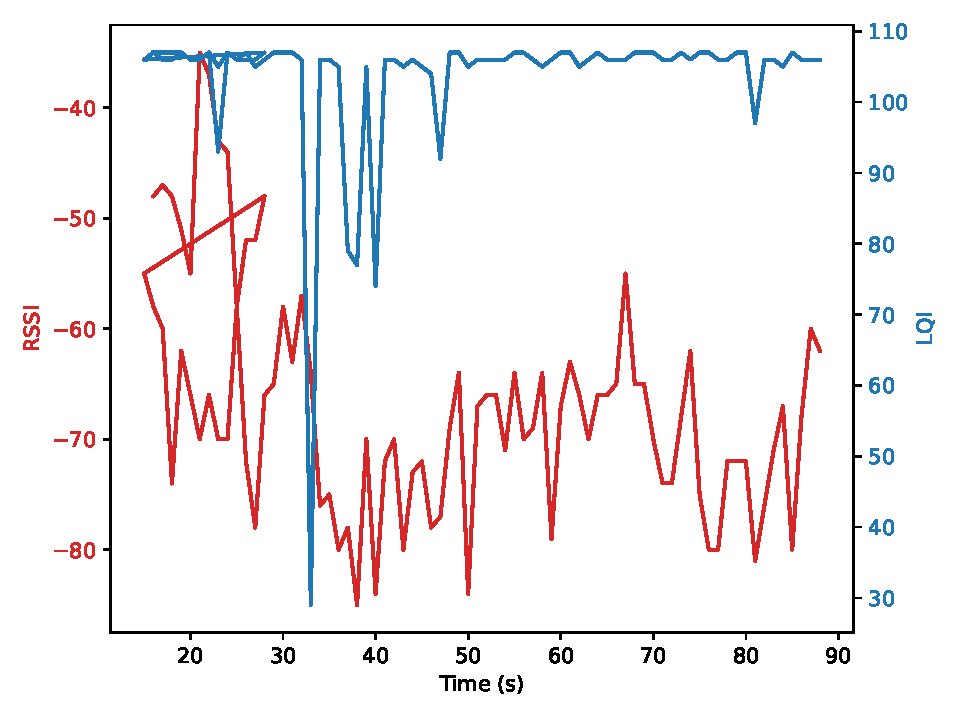
\includegraphics[width=\textwidth]{images/1-50-7-26-line.pdf}
        \caption{Line plot}
    \end{subfigure}
    \hfill
    \begin{subfigure}[b]{0.45\textwidth}
        \centering
        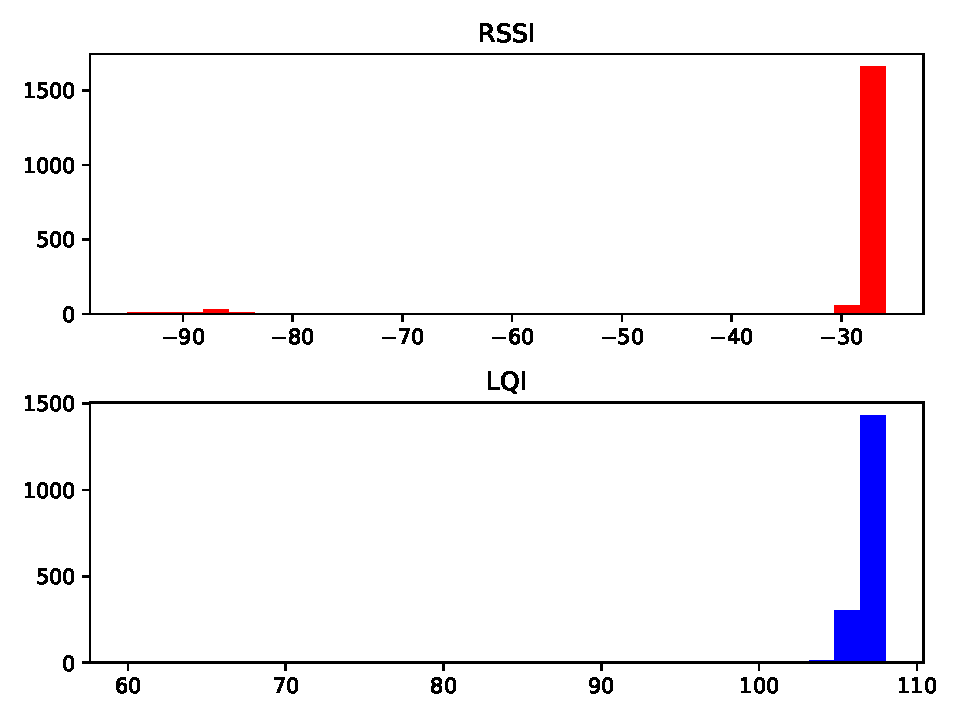
\includegraphics[width=\textwidth]{images/1-50-7-26-histogram.pdf}
        \caption{Histogram plot}
    \end{subfigure}
    \caption{Plots for Test 4}
\end{figure}

\begin{figure}[ht]
    \centering
    \begin{subfigure}[b]{0.45\textwidth}
        \centering
        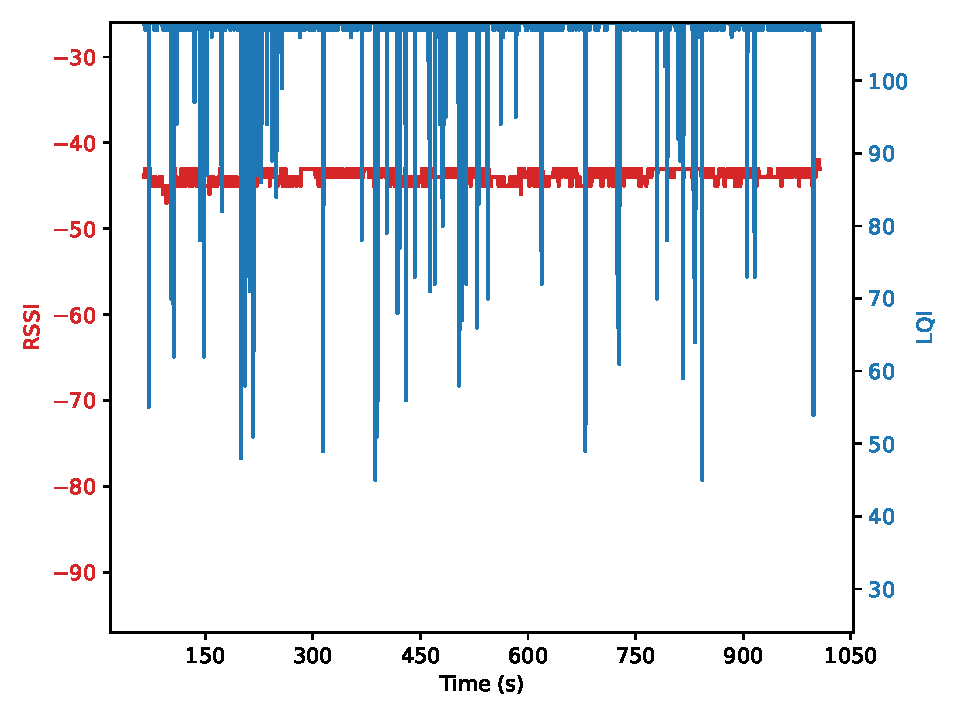
\includegraphics[width=\textwidth]{images/1-50-0-11-line.pdf}
        \caption{Line plot}
    \end{subfigure}
    \hfill
    \begin{subfigure}[b]{0.45\textwidth}
        \centering
        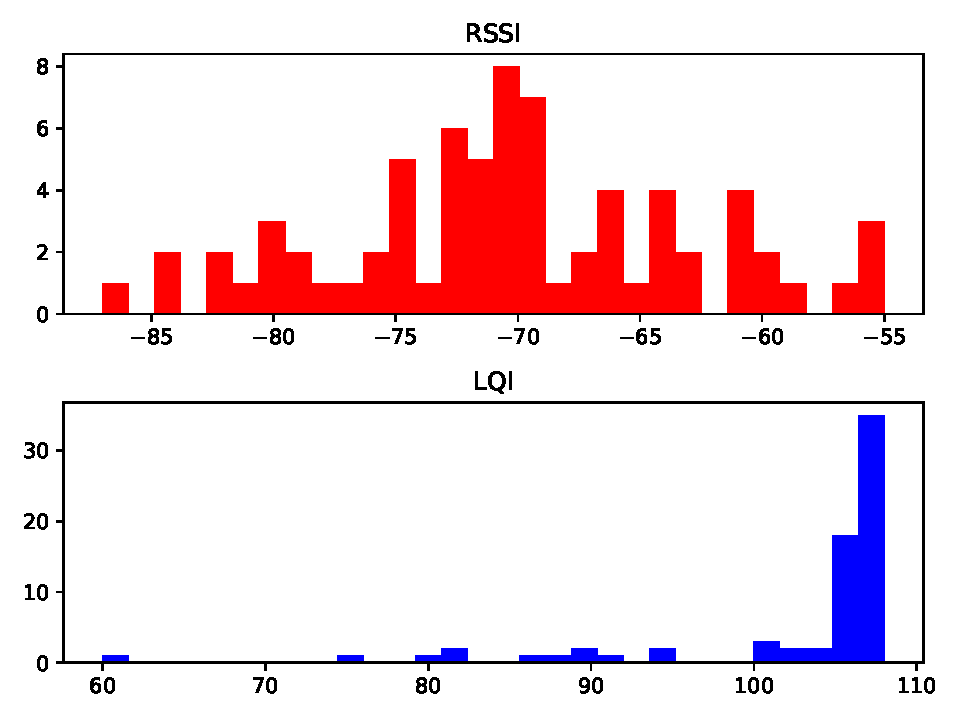
\includegraphics[width=\textwidth]{images/1-50-0-11-histogram.pdf}
        \caption{Histogram plot}
    \end{subfigure}
    \caption{Plots for Test 5}
\end{figure}

\begin{figure}[ht]
    \centering
    \begin{subfigure}[b]{0.45\textwidth}
        \centering
        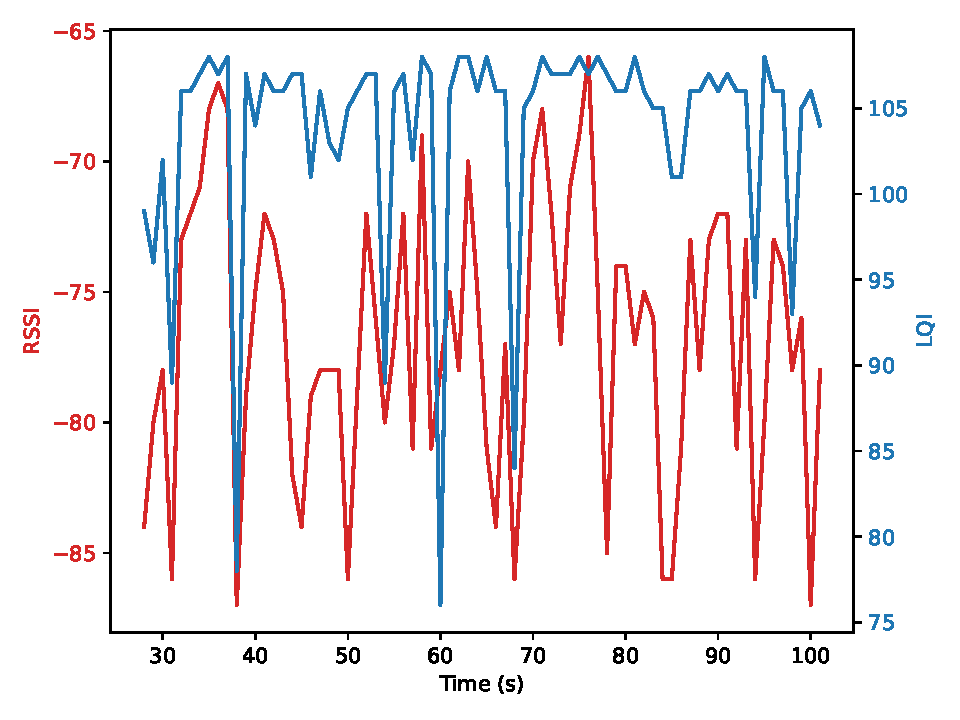
\includegraphics[width=\textwidth]{images/1-50-0-15-line.pdf}
        \caption{Line plot}
    \end{subfigure}
    \hfill
    \begin{subfigure}[b]{0.45\textwidth}
        \centering
        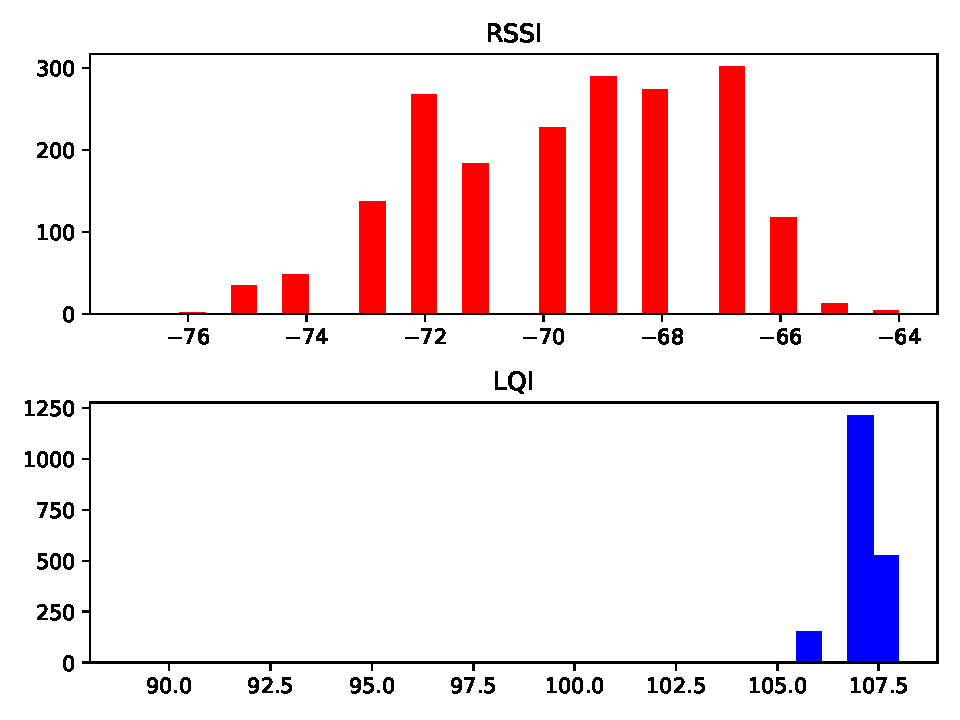
\includegraphics[width=\textwidth]{images/1-50-0-15-histogram.pdf}
        \caption{Histogram plot}
    \end{subfigure}
    \caption{Plots for Test 6}
\end{figure}

\begin{figure}[ht]
    \centering
    \begin{subfigure}[b]{0.45\textwidth}
        \centering
        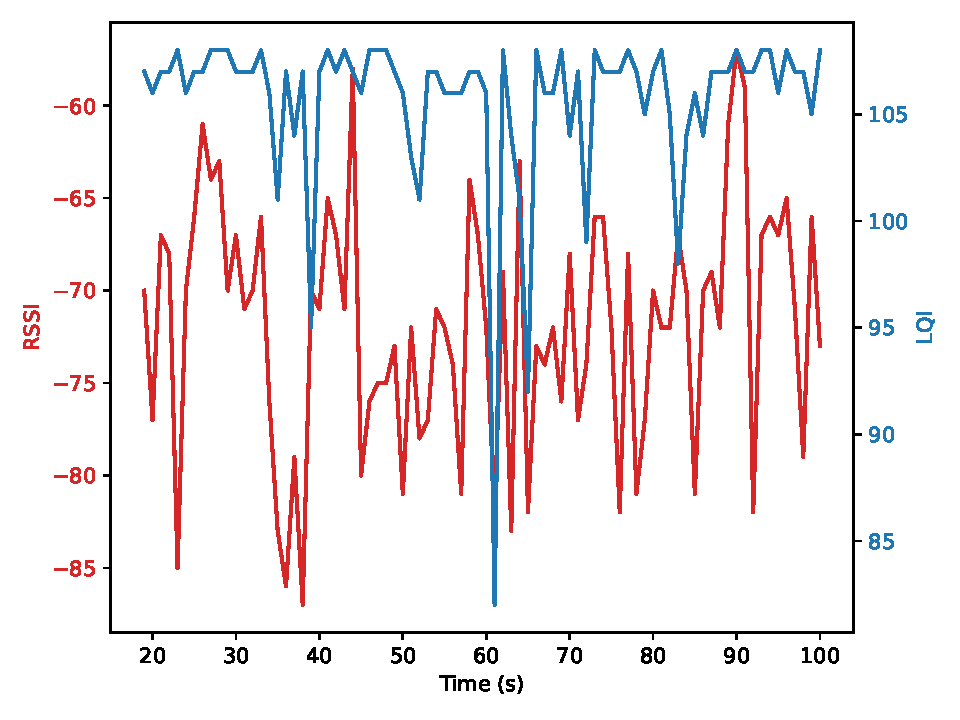
\includegraphics[width=\textwidth]{images/1-50-0-20-line.pdf}
        \caption{Line plot}
    \end{subfigure}
    \hfill
    \begin{subfigure}[b]{0.45\textwidth}
        \centering
        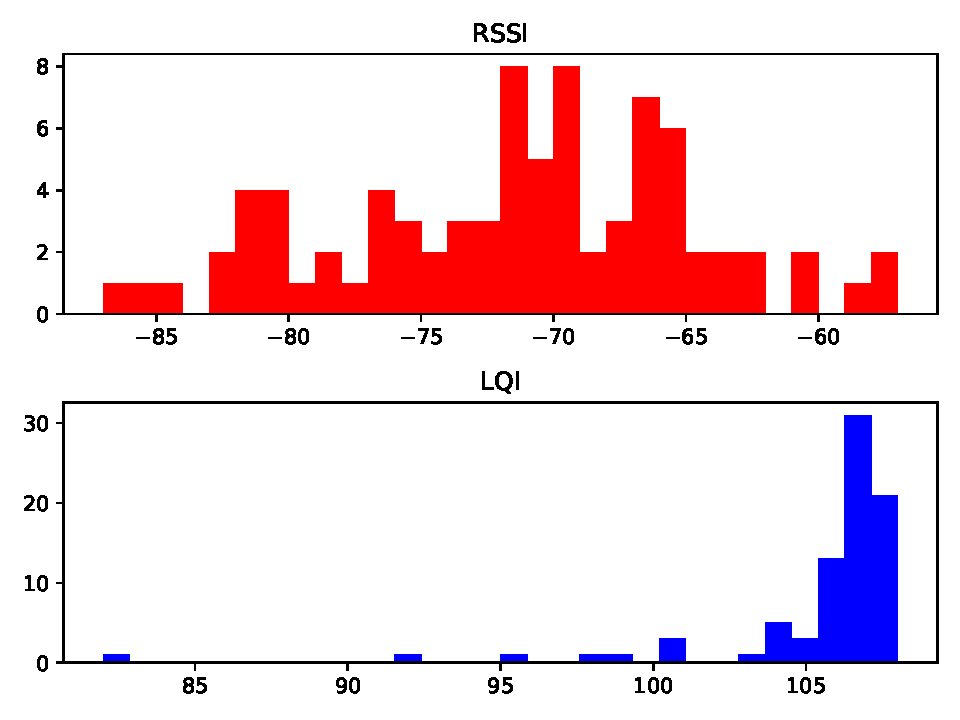
\includegraphics[width=\textwidth]{images/1-50-0-20-histogram.pdf}
        \caption{Histogram plot}
    \end{subfigure}
    \caption{Plots for Test 7}
\end{figure}

\begin{figure}[ht]
    \centering
    \begin{subfigure}[b]{0.45\textwidth}
        \centering
        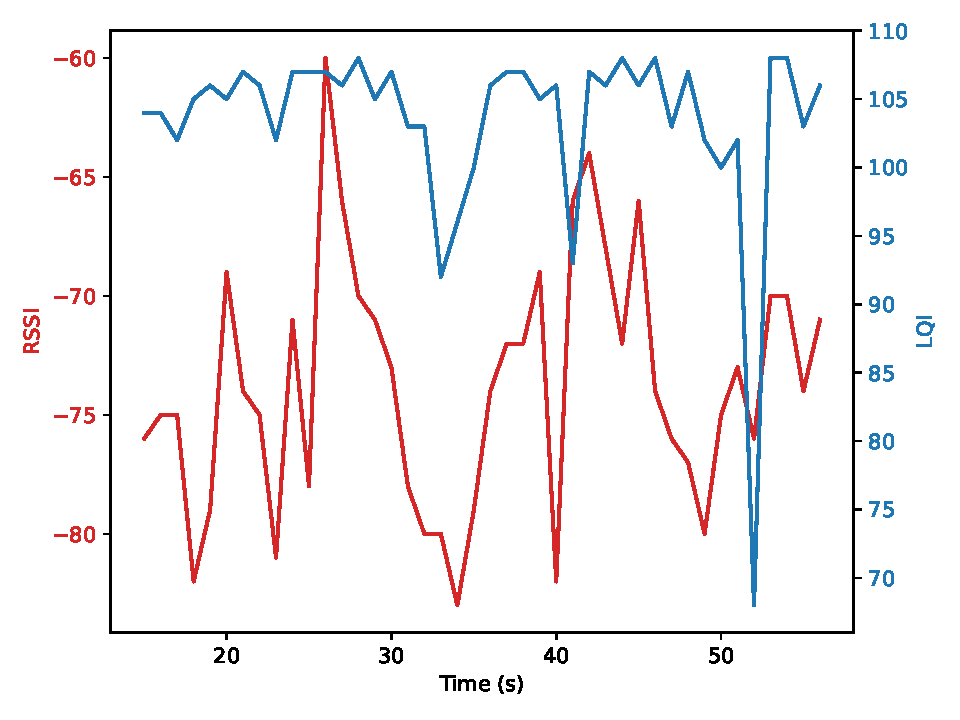
\includegraphics[width=\textwidth]{images/1-20-0-26-line.pdf}
        \caption{Line plot}
    \end{subfigure}
    \hfill
    \begin{subfigure}[b]{0.45\textwidth}
        \centering
        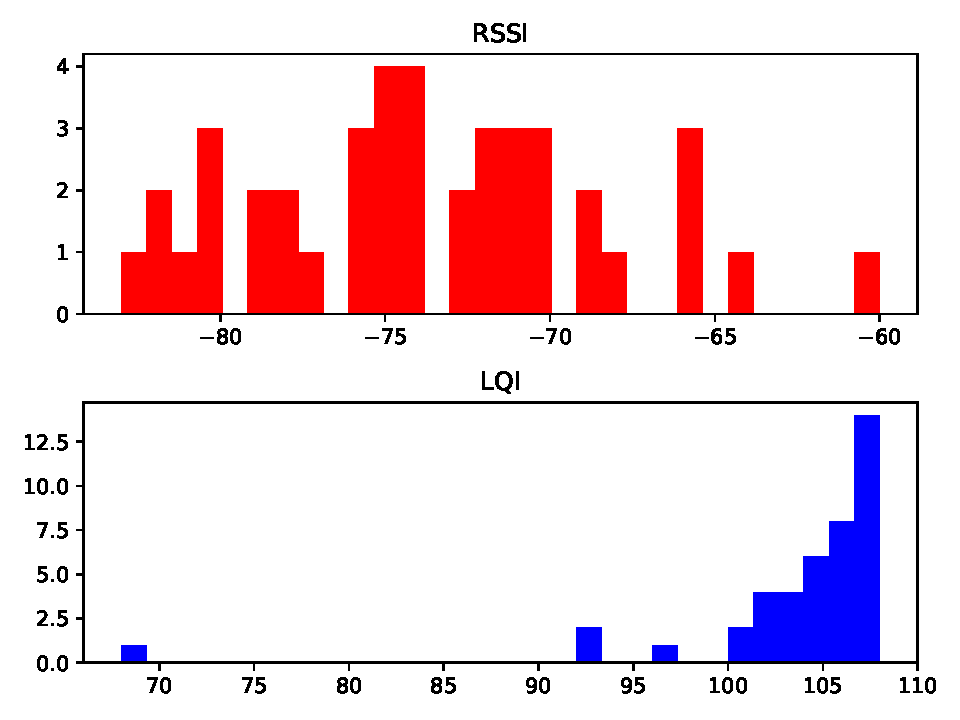
\includegraphics[width=\textwidth]{images/1-20-0-26-histogram.pdf}
        \caption{Histogram plot}
    \end{subfigure}
    \caption{Plots for Test 8}
\end{figure}

\begin{figure}[ht]
    \centering
    \begin{subfigure}[b]{0.45\textwidth}
        \centering
        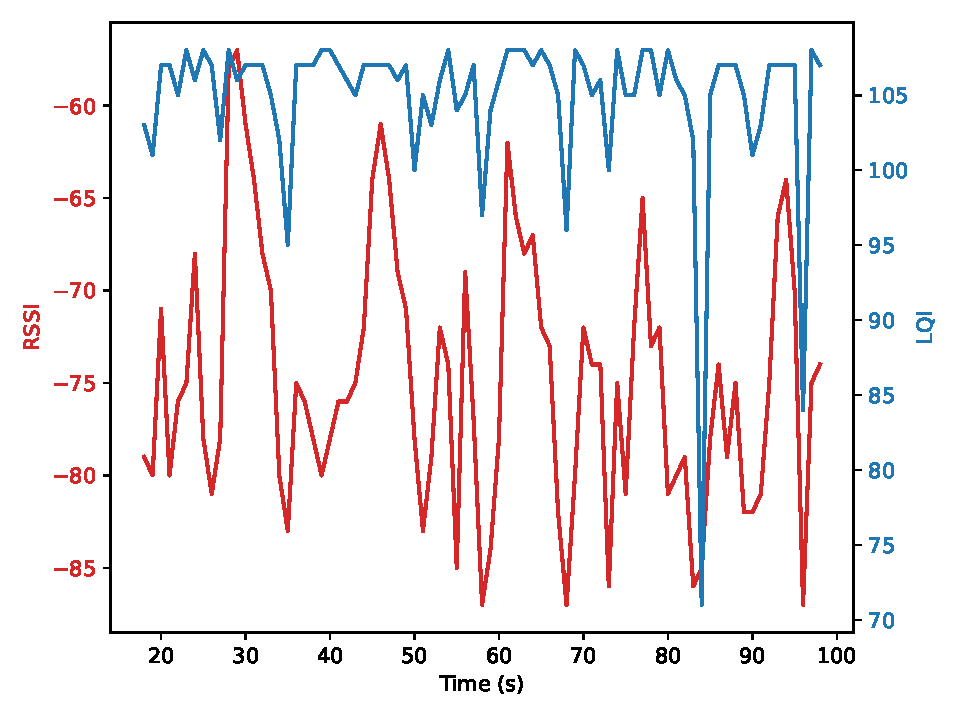
\includegraphics[width=\textwidth]{images/1-100-0-26-line.pdf}
        \caption{Line plot}
    \end{subfigure}
    \hfill
    \begin{subfigure}[b]{0.45\textwidth}
        \centering
        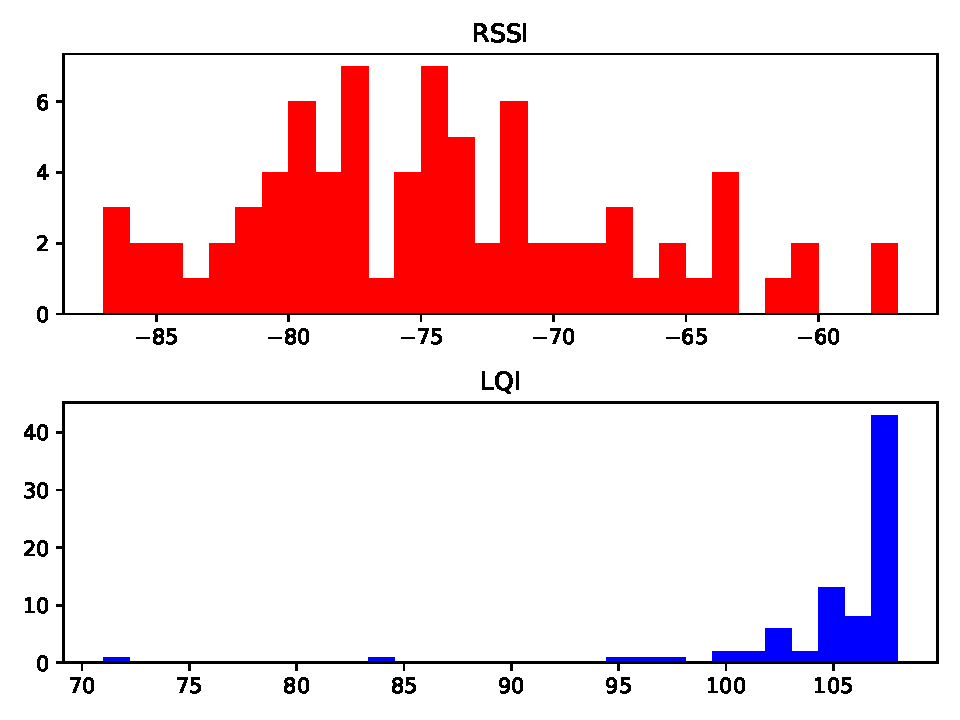
\includegraphics[width=\textwidth]{images/1-100-0-26-histogram.pdf}
        \caption{Histogram plot}
    \end{subfigure}
    \caption{Plots for Test 9}
\end{figure}

\clearpage

The experimental evaluation yielded noteworthy results concerning the impact of the transmission power, transmission channel, and packet size on multi-hop packet transmission. The results for each of the parameter changes are discussed in detail below.

\subsection{Impact of Transmission Power}

Our experiments showed that varying the transmission power had the most significant impact on the results. As the transmission power was decreased (Tests 2 and 3), there was a notable decline in the Link Quality Indicator (LQI) and Received Signal Strength Indicator (RSSI) values. This was expected, as a lower transmission power typically leads to a weaker signal at the receiver, thereby reducing the signal quality. This effect was accentuated when the distance between the nodes increased slightly, leading to a loss of connection, which underscored the importance of adequate transmission power in maintaining connectivity in a mobile wireless sensor network.

Conversely, increasing the transmission power (Test 4) led to higher LQI and RSSI values, indicating improved signal quality. However, the values were extremely unstable, fluctuating drastically from one packet to the next. This volatility can be attributed to several factors, including interference from other devices, multi-path fading due to the mobility of the bicycles, and changing environmental conditions.

\subsection{Impact of Transmission Channel}

Altering the transmission channel also significantly impacted the results, but not as dramatically as changes to the transmission power. The transmission channel, which defines the frequency band used for communication, can greatly affect the noise in the signal, and thus the quality of the received packets. In the presence of other devices operating on the same or nearby frequencies, changing the channel can help avoid interference and improve communication reliability. However, the choice of channel can also be influenced by environmental factors, as signal propagation characteristics can vary with frequency.

Tests 5, 6, and 7 explored the impact of using different transmission channels. The results showed that the LQI and RSSI values were slightly more stable compared to the transmission power tests, suggesting less interference and more consistent signal propagation conditions on the chosen channels. We did find that the LQI and RSSI values were more stable on the default channel (26) in comparison with the other channels (11, 15, and 20). This indicates that the default channel is more suitable for the bicycle network scenario.

% compared to the other channels, which is likely due to the fact that the default channel is less prone to interference from other devices.

\subsection{Impact of Packet Size}

Finally, varying the packet size had the least impact on the results, with the LQI and RSSI values remaining relatively stable throughout the experiments (Tests 8 and 9). However, it was observed that smaller packet sizes yielded slightly better results, likely due to the reduced probability of packet errors in shorter transmissions.

\subsection{Inter Packet Interval}

We also experimented with the inter packet interval (IPI), but due to the limitations of the timer we chose for our implementation (the \texttt{etimer} module), we were unable to set the IPI to a value lower than 1 second. This meant that we were unable to draw any conclusions from the results, as the IPI was too high to be able to observe any significant changes in the LQI and RSSI values.

In summary, our experiments have shown that in a mobile multi-hop wireless sensor network, the transmission power significantly impacts the quality of packet transmission, followed by the choice of transmission channel. Packet size, while not as impactful, can also affect the transmission quality, particularly in noisy or interference-prone environments. These findings underline the importance of carefully configuring these parameters to ensure reliable communication in mobile wireless sensor networks. Future research could explore the impact of other parameters, such as modulation scheme, error correction techniques, and network topology, on multi-hop packet transmission.

\section{Conclusion}

In conclusion, our investigation has provided valuable insights into the impact of various parameters on multi-hop packet transmission in a mobile wireless sensor network. We found that transmission power had the most profound impact on the packet transmission quality, with both the LQI and RSSI values being highly sensitive to changes in this parameter. Transmission channel and packet size also played important roles, albeit to a lesser extent.

The findings underline the importance of carefully configuring these parameters when setting up a mobile wireless sensor network. It is worth noting that while our study focused on a specific scenario involving bicycles, the insights gained are expected to be applicable to a broader range of mobile network scenarios.

%
% ---- Bibliography ----
%
% BibTeX users should specify bibliography style 'splncs04'.
% References will then be sorted and formatted in the correct style.
%
% \bibliographystyle{splncs04}
% \bibliography{mybibliography}
%

\bibliographystyle{splncs04}
\bibliography{references}

\end{document}